\documentclass[12pt,addpoints]{repaso}
\grado{6}
\nivel{Primaria}
\cicloescolar{2024-2025}
\materia{Matemáticas}
\unidad{2}
\title{Practica la Unidad}
\aprendizajes{\scriptsize%
% \item Estudio de los números.
\item Expresa oralmente la sucesión numérica hasta billones, en español y hasta donde sea posible, en su lengua materna, de manera ascendente y descendente a partir de un número natural dado. Ordena, lee y escribe números naturales de más de nueve cifras e interpreta números decimales en diferentes contextos. Identifica semejanzas y diferencias entre el sistema de numeración decimal y otros sistemas como el maya y el romano\\[-1.5em]
	% \item Suma y resta, su relación como operaciones inversas.
	\item A partir de situaciones problemáticas vinculadas a diferentes contextos, suma y resta números decimales y fracciones con diferentes denominadores.\\[-1.5em]
	% \item Multiplicación y división, su relación como operaciones inversas.
	\item Resuelve situaciones problemáticas vinculadas a diferentes contextos que implican dividir números decimales entre naturales. También, dividir números fraccionarios entre números naturales.\\[-1.5em]
	% \item Relaciones de proporcionalidad.
	\item A partir de situaciones problemáticas de proporcionalidad vinculadas a diferentes contextos, determina valores faltantes en las que en ocasiones se conoce el valor unitario y en otras no.\\[-1.5em]
	% \item Ubicación espacial.
	\item Lee, interpreta y elabora planos para comunicar la ubicación de seres vivos y objetos.\\[-1.5em]
	% \item Figuras y cuerpos geométricos y sus características.
	\item Explora y reconoce las características del cilindro y cono; anticipa y comprueba desarrollos planos que permiten construirlos.\\[-1.5em]
	% \item Perímetro, área y noción de volumen.
	\item Resuelve situaciones problemáticas que implican calcular el perímetro y área de figuras compuestas por triángulos y cuadriláteros. Resuelve problemas que implican construir, estimar y comparar el volumen de cuerpos y prismas rectos rectangulares mediante el conteo de cubos, y reconoce que existen diferentes cuerpos con el mismo volumen.\\[-1.5em]
	% \item Organización e interpretación de datos.
	\item Interpreta información cuantitativa y cualitativa contenida en tablas, gráficas de barras y circulares para responder preguntas vinculadas a diferentes contextos; construye gráficas de barras. Genera y organiza datos, determina la moda, la media aritmética y el rango para responder preguntas vinculadas a diferentes contextos.\\[-1.5em]
	% \item Nociones de probabilidad.
	\item Clasifica eventos de diversos contextos utilizando términos como seguro, imposible, probable, muy probable o poco probable que sucedan.
}
\author{Melchor Pinto, JC}
\begin{document}
\INFO\afterpage{\blankpage}%

\begin{multicols}{2}
	\tableofcontents
\end{multicols}

\begin{questions}\large

		\addcontentsline{toc}{section}{Unidad 2}
	\section*{Unidad 2}

	\addcontentsline{toc}{subsection}{Introducción a fracciones}
	\subsection*{Introducción a fracciones}
	\addcontentsline{toc}{subsubsection}{Clasificación de fracciones}
	\subsubsection*{Clasificación de fracciones}

	\questionboxed[2]{Clasifica las siguientes fracciones en propias, impropias o mixtas:

		\begin{multicols}{4}
			\begin{parts}
				\part $\dfrac{5}{6}$   \fillin[Propia][1in]     \\[0.5em]
				\part $5\dfrac{5}{11}$ \fillin[Mixta][1in]      \\[0.5em]
				\part $\dfrac{13}{12}$   \fillin[Impropia][1in] \\[0.5em]
				\part $1\dfrac{2}{15}$  \fillin[Mixta][1in]     \\[0.5em]
				\part $\dfrac{42}{43}$   \fillin[Propia][1in]   \\[0.5em]
				\part $\dfrac{16}{9}$   \fillin[Impropia][1in]  \\[0.5em]
				\part $\dfrac{7}{3}$   \fillin[Impropia][1in]   \\[0.5em]
				\part $3\dfrac{2}{9}$  \fillin[Mixta][1in]      \\[0.5em]
				\part $\dfrac{3}{2}$   \fillin[Impropia][1in]   \\[0.5em]
				\part $1\dfrac{2}{3}$  \fillin[Mixta][1in]      \\[0.5em]
				\part $\dfrac{7}{8}$   \fillin[Propia][1in]     \\[0.5em]
				\part $\dfrac{6}{5}$   \fillin[Impropia][1in]   \\[0.5em]
			\end{parts}
		\end{multicols}
	}

	\addcontentsline{toc}{subsubsection}{Representación de fracciones}
	\subsubsection*{Representación de fracciones}

	\questionboxed[2]{Escribe sobre la línea la fracción que representa cada imagen:

		\begin{multicols}{4}
			\begin{parts}
				\part 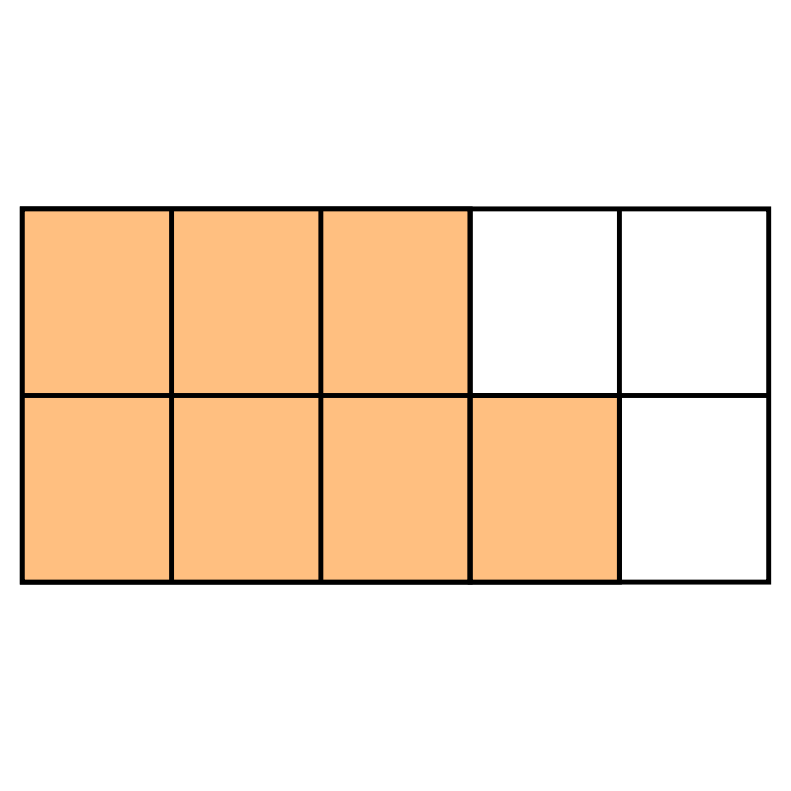
\includegraphics[width=50px]{../images/imagen_frac_5prim_7|10.png} \fillin[\fbox{$\dfrac{7}{10}$}][0in] \\[-0.5em]
				\part 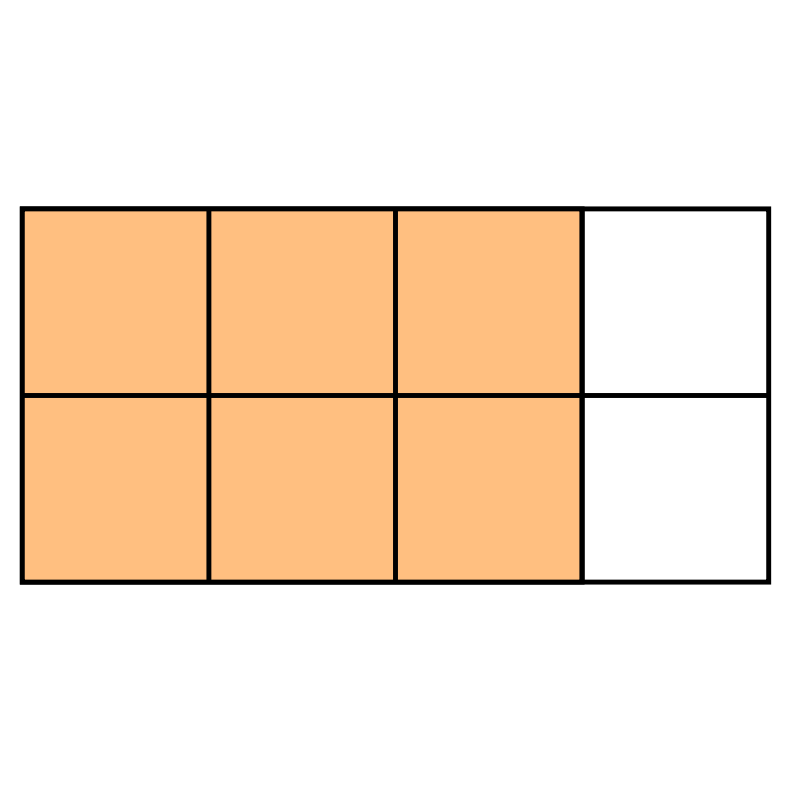
\includegraphics[width=50px]{../images/imagen_frac_5prim_6|8.png} \fillin[\fbox{$\dfrac{6}{8}$}][0in] \\[-0.5em]
				\part 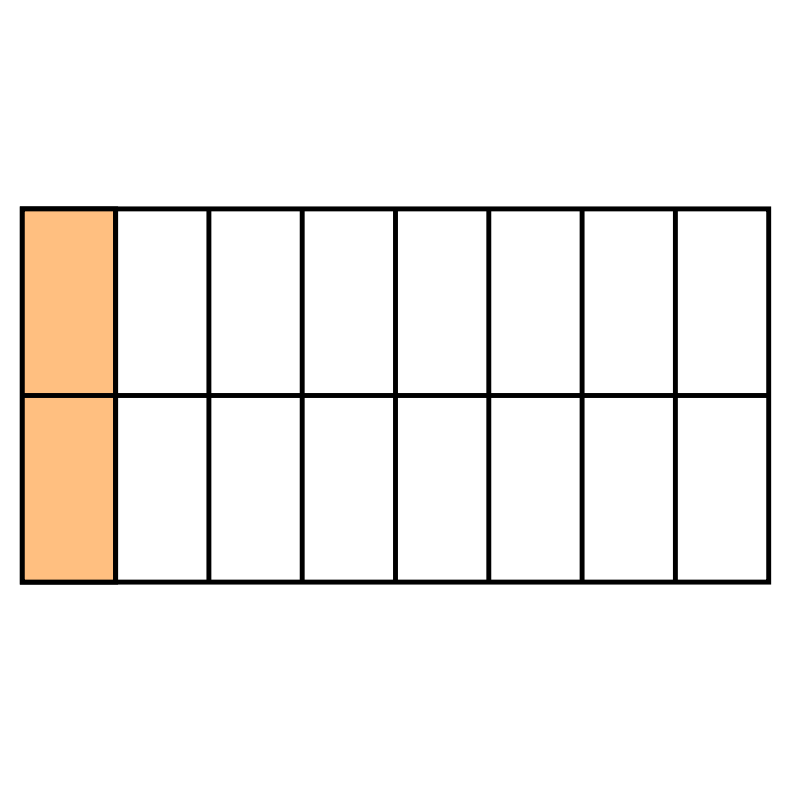
\includegraphics[width=50px]{../images/imagen_frac_5prim_2|16.png} \fillin[\fbox{$\dfrac{2}{16}$}][0in] \\[-0.5em]
				% \part 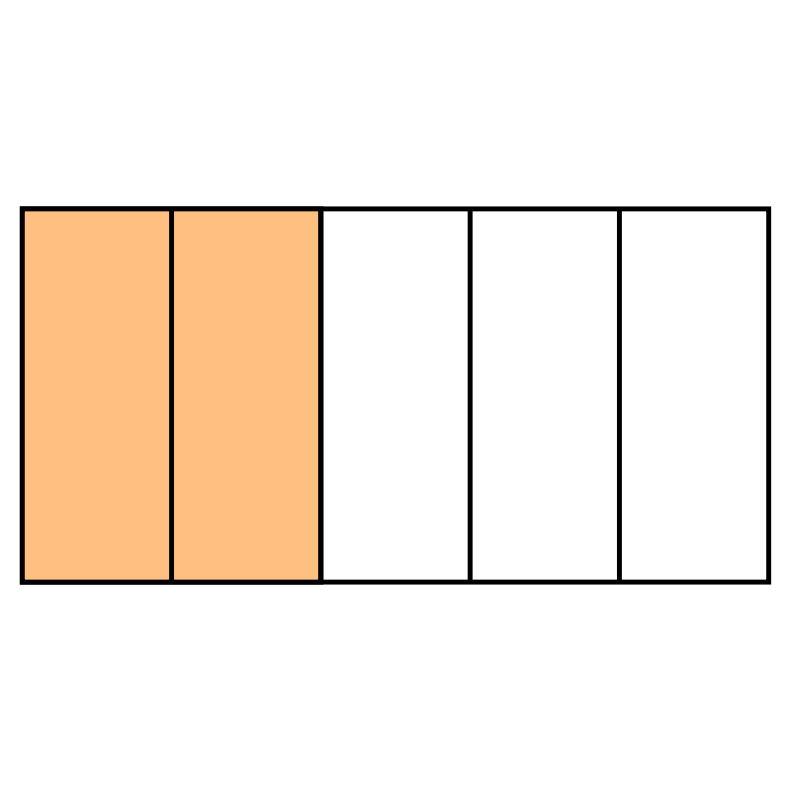
\includegraphics[width=50px]{../images/imagen_frac_5prim_2|5.png} \fillin[\fbox{$\dfrac{2}{5}$}][0in] \\[-0.5em]
				\part 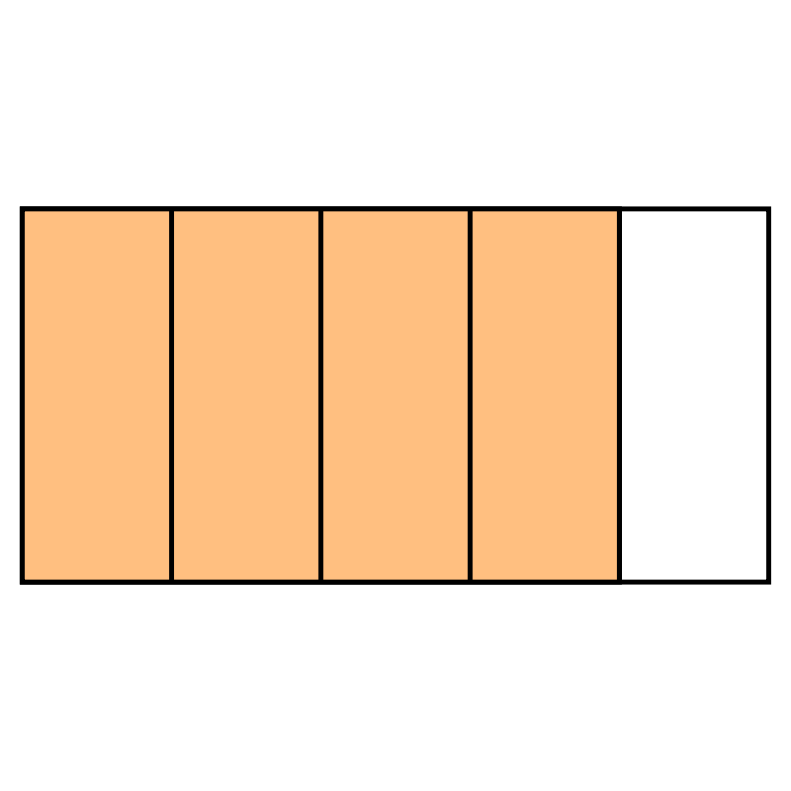
\includegraphics[width=50px]{../images/imagen_frac_5prim_4|5.png} \fillin[\fbox{$\dfrac{4}{5}$}][0in] \\[-0.5em]
				% \part 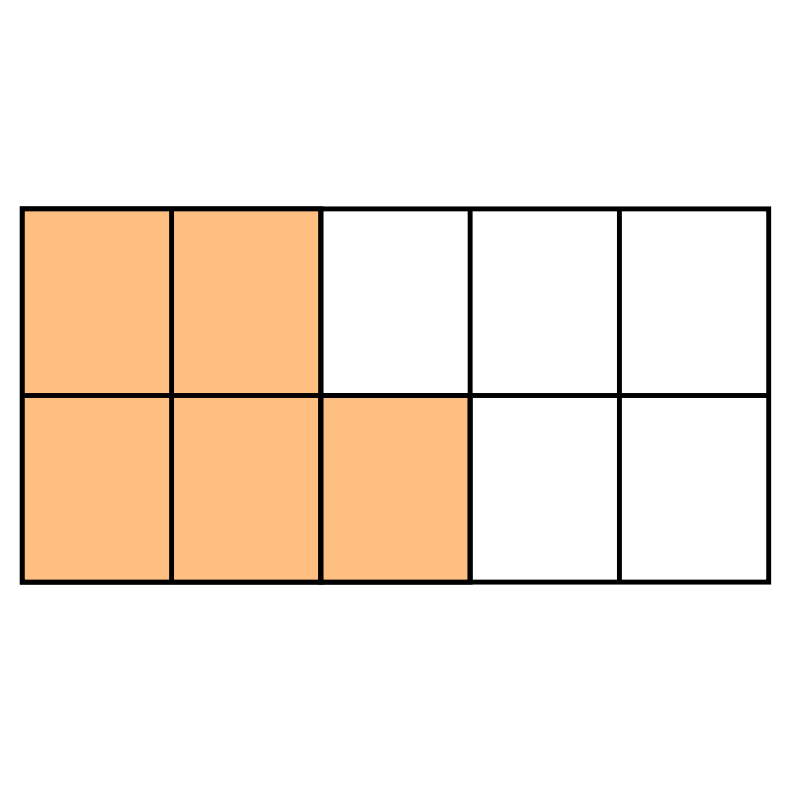
\includegraphics[width=50px]{../images/imagen_frac_5prim_5|10.png} \fillin[\fbox{$\dfrac{5}{10}$}][0in] \\[-0.5em]
				% \part 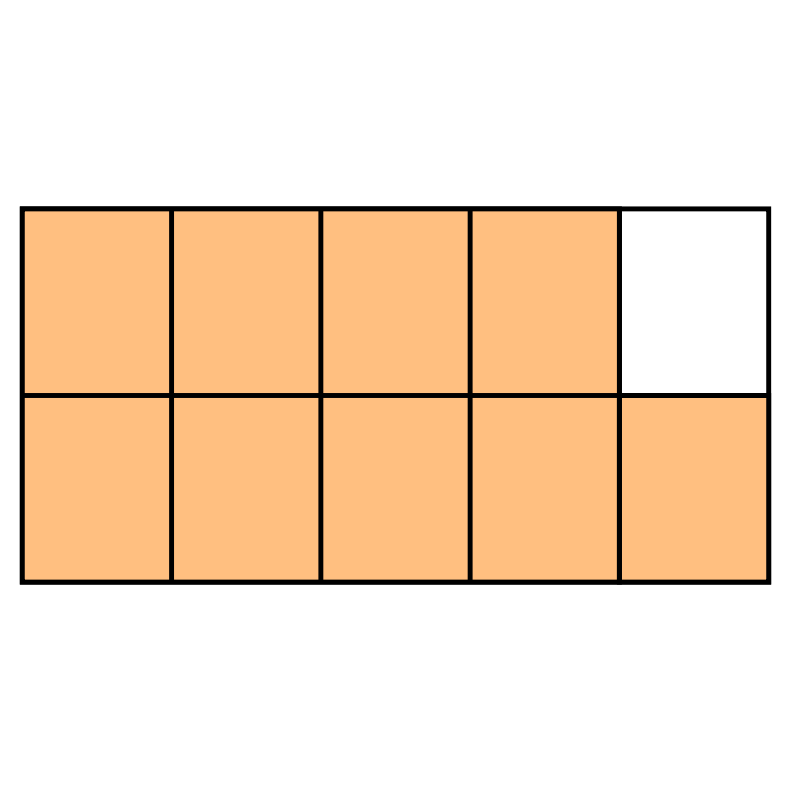
\includegraphics[width=50px]{../images/imagen_frac_5prim_9|10.png} \fillin[\fbox{$\dfrac{9}{10}$}][0in] \\[-0.5em]
				% \part 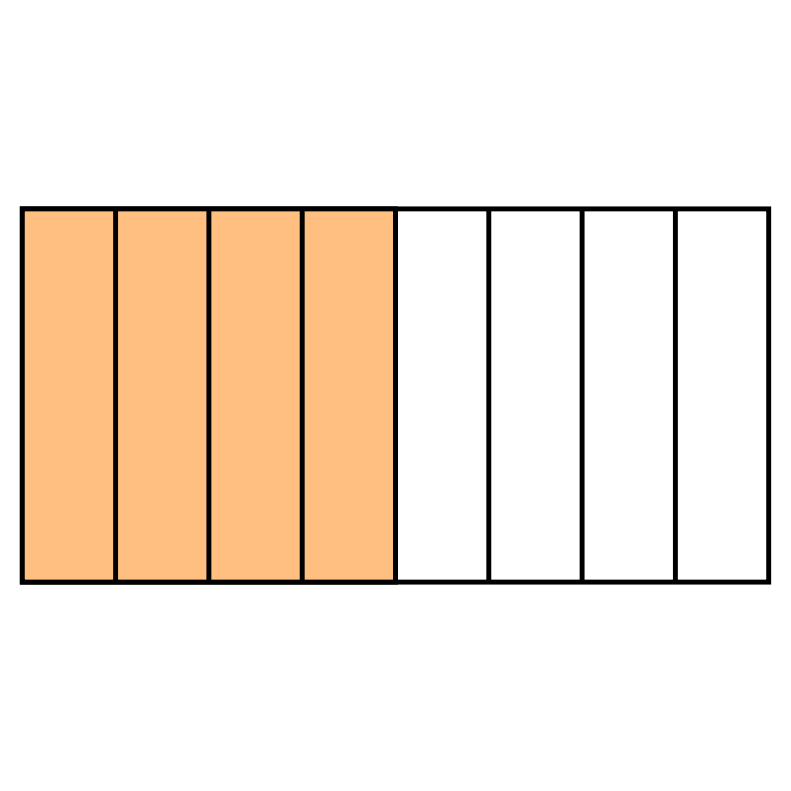
\includegraphics[width=50px]{../images/imagen_frac_5prim_4|8.png} \fillin[\fbox{$\dfrac{4}{8}$}][0in] \\[-0.5em]
				% \part 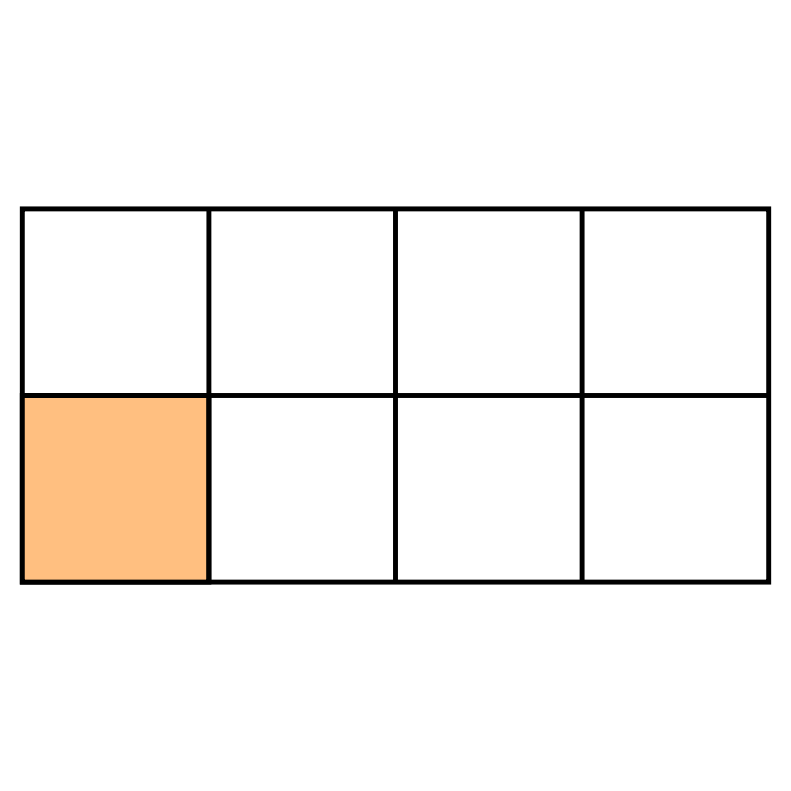
\includegraphics[width=50px]{../images/imagen_frac_5prim_1|8.png} \fillin[\fbox{$\dfrac{1}{8}$}][0in] \\[-0.5em]
				\part 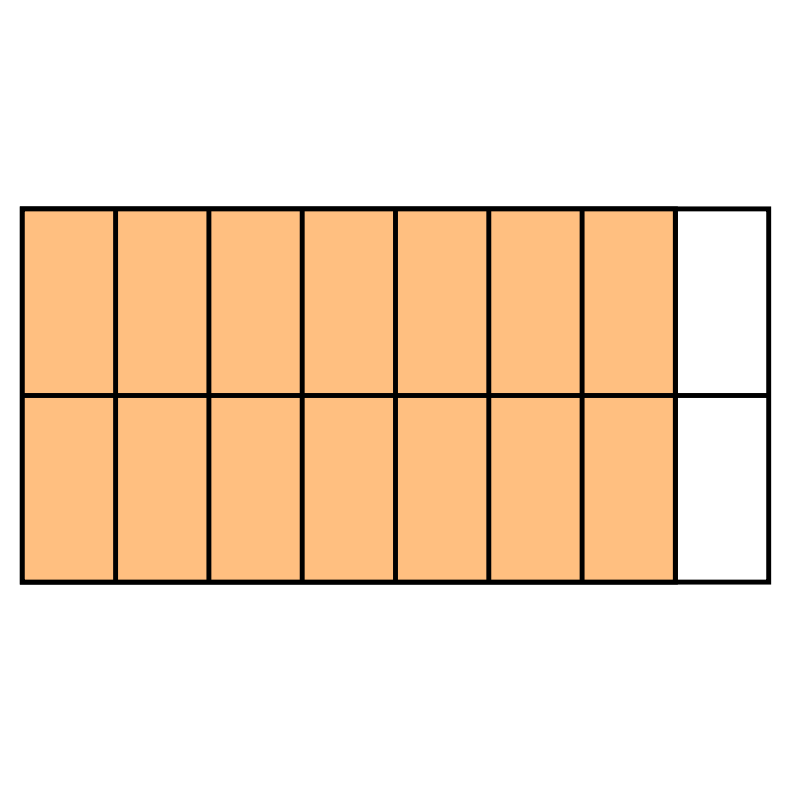
\includegraphics[width=50px]{../images/imagen_frac_5prim_14|16.png} \fillin[\fbox{$\dfrac{14}{16}$}][0in] \\[-0.5em]
				% \part 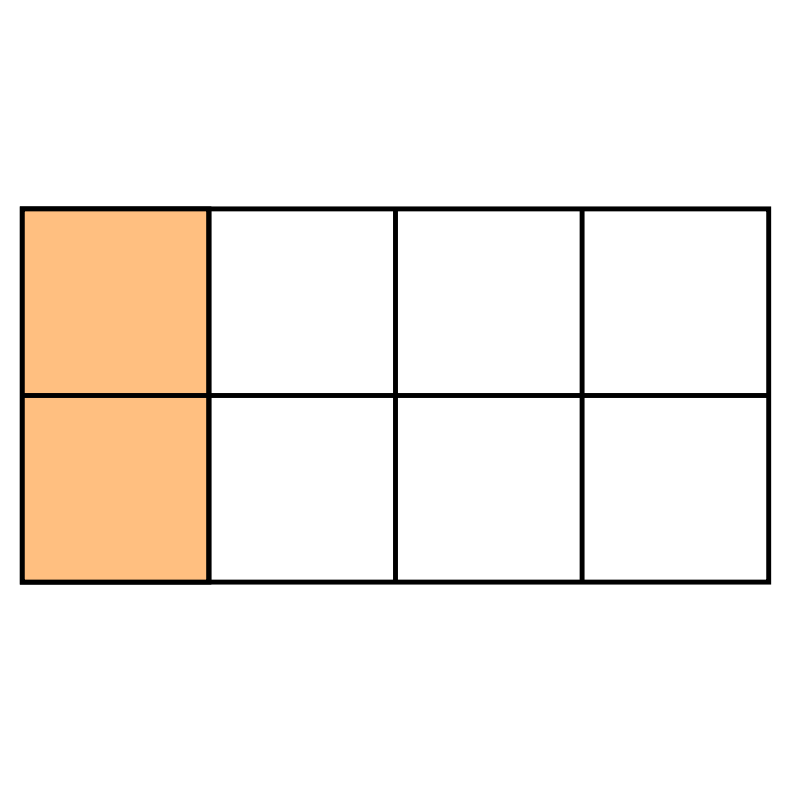
\includegraphics[width=50px]{../images/imagen_frac_5prim_2|8.png} \fillin[\fbox{$\dfrac{2}{8}$}][0in] \\[-0.5em]
				\part 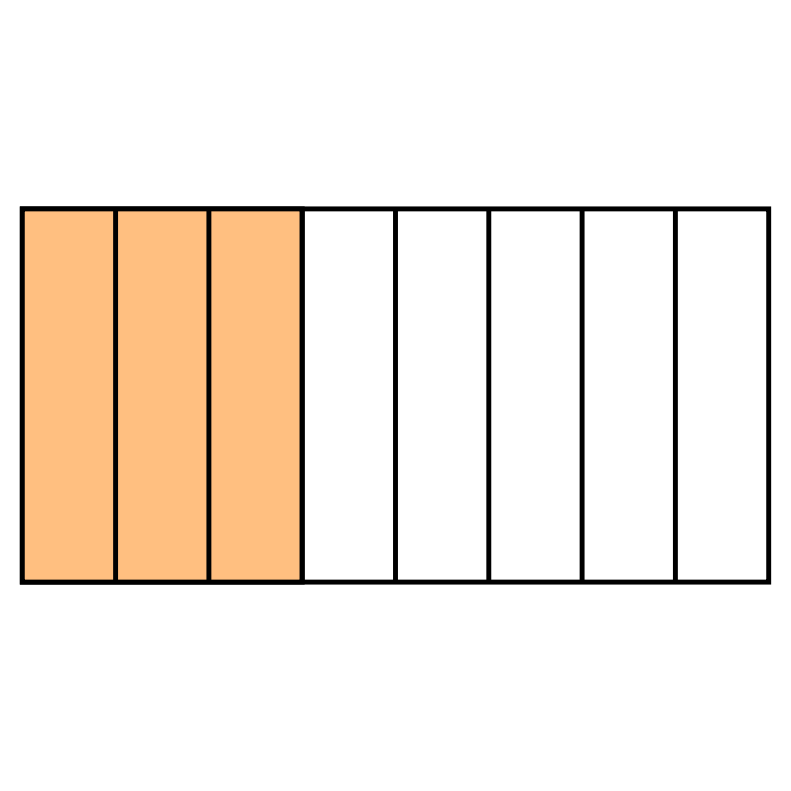
\includegraphics[width=50px]{../images/imagen_frac_5prim_3|8.png} \fillin[\fbox{$\dfrac{3}{8}$}][0in] \\[-0.5em]
				\part 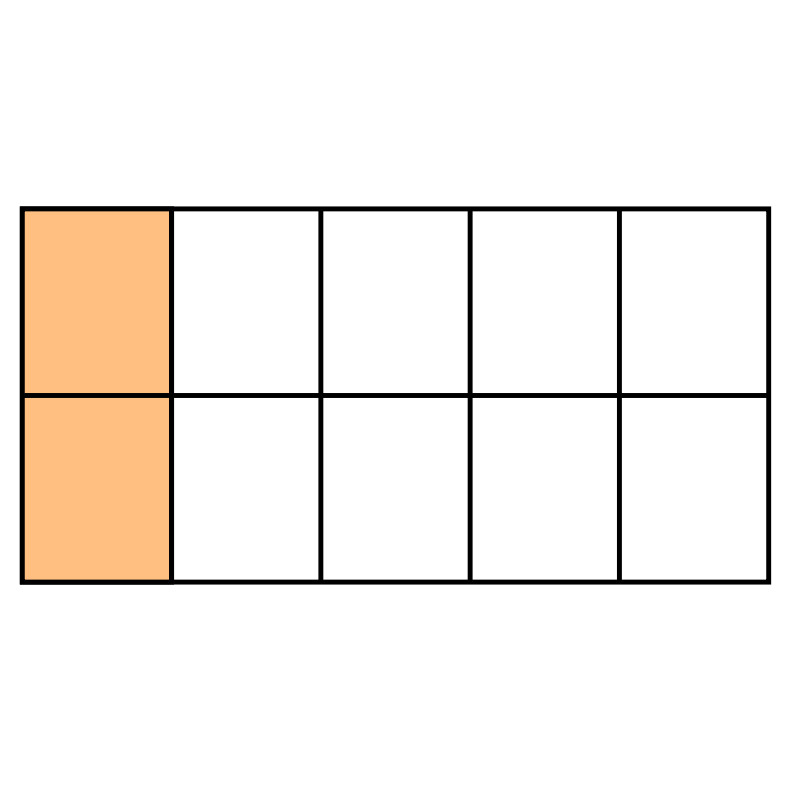
\includegraphics[width=50px]{../images/imagen_frac_5prim_2|10.png} \fillin[\fbox{$\dfrac{2}{10}$}][0in] \\[-0.5em]
				\part 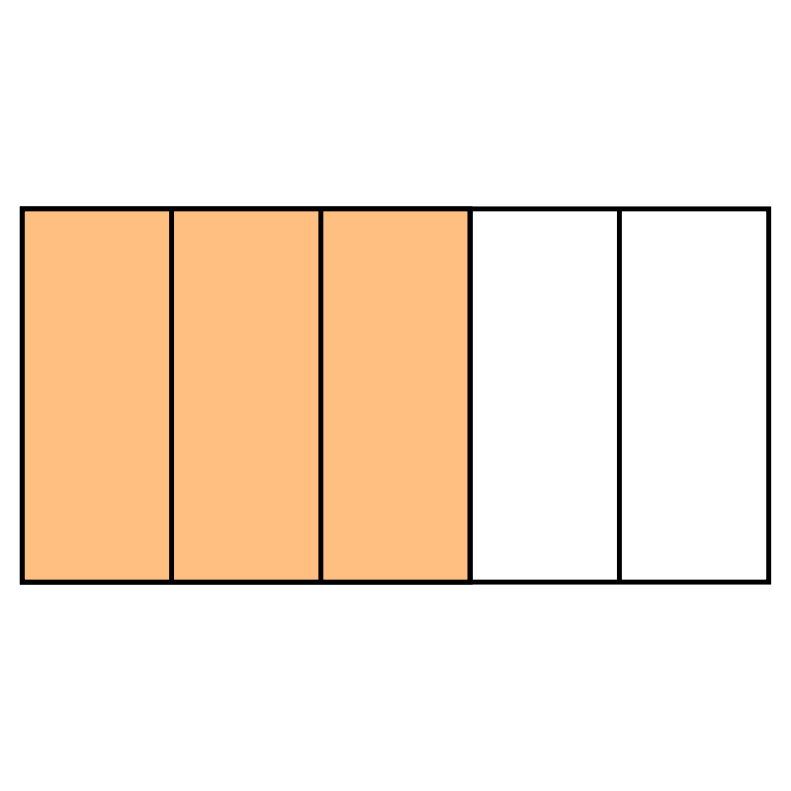
\includegraphics[width=50px]{../images/imagen_frac_5prim_3|5.png} \fillin[\fbox{$\dfrac{3}{5}$}][0in] \\[-0.5em]
				% \part 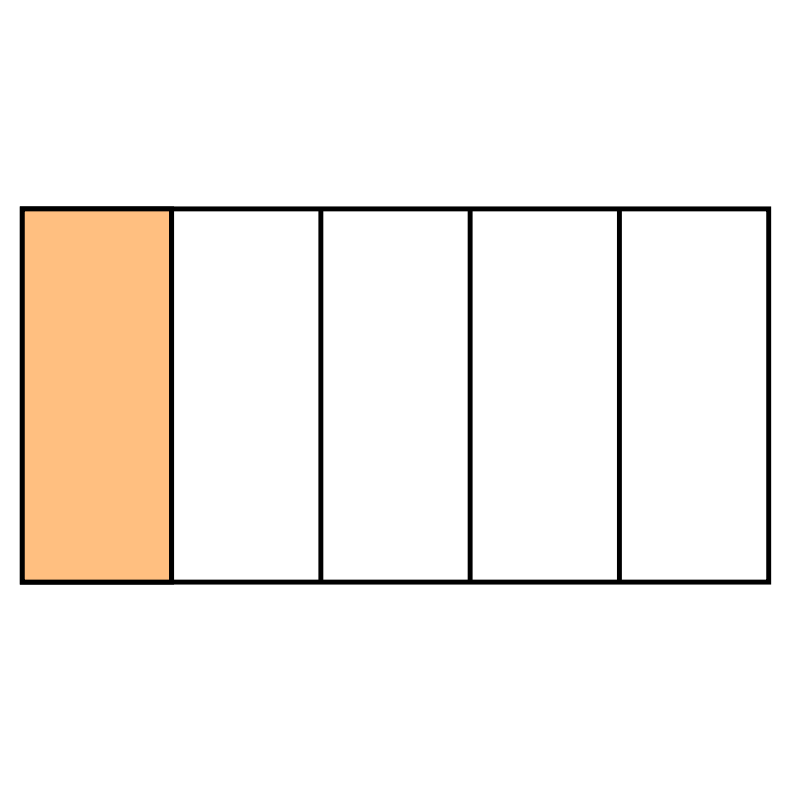
\includegraphics[width=50px]{../images/imagen_frac_5prim_1|5.png} \fillin[\fbox{$\dfrac{1}{5}$}][0in] \\[-0.5em]
				% \part 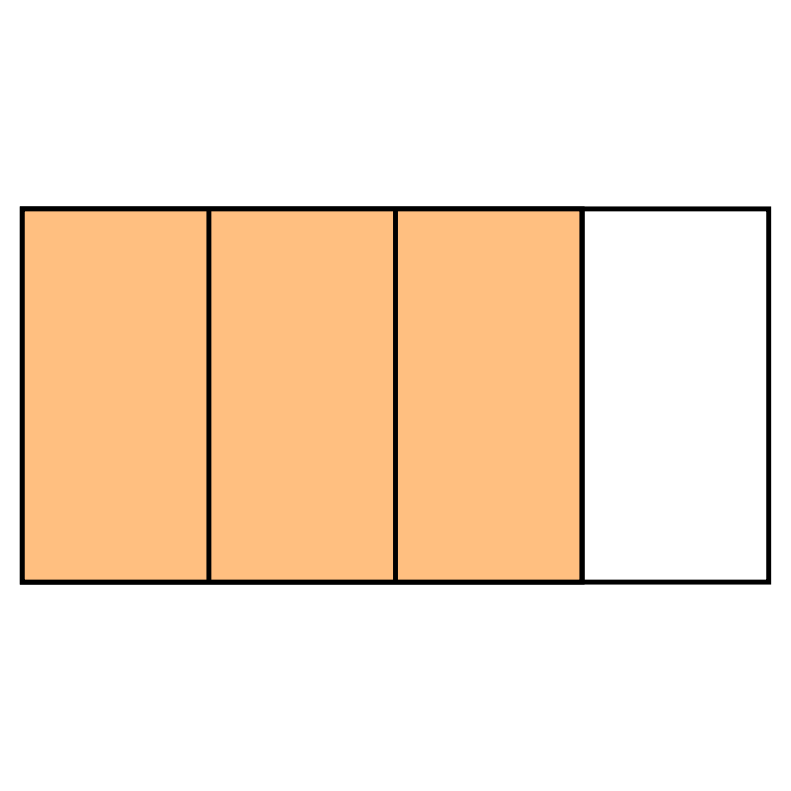
\includegraphics[width=50px]{../images/imagen_frac_5prim_3|4.png} \fillin[\fbox{$\dfrac{3}{4}$}][0in] \\[-0.5em]
			\end{parts}
		\end{multicols}
	}

	\addcontentsline{toc}{subsubsection}{Nombre de fracciones}
	\subsubsection*{Nombre de fracciones}

	\questionboxed[2]{Escribe la fracción que corresponda en cada inciso:

		\begin{parts}
			\part ¿Cómo se escribe numéricamente la fracción \textbf{siete catorceavos}?    \fillin[$\dfrac{7}{14}$][0in]
			\part ¿Cómo se escribe numéricamente la fracción \textbf{ocho onceavos}?   \fillin[$\dfrac{8}{11}$][0in]
			\part ¿Cómo se escribe numéricamente la fracción \textbf{doce séptimos}?    \fillin[$\dfrac{12}{7}$][0in]
			\part ¿Cómo se escribe numéricamente la fracción \textbf{nueve treceavos}?     \fillin[$\dfrac{9}{13}$][0in]
		\end{parts}
	}

	\addcontentsline{toc}{subsubsection}{Fracciones en la recta numérica}
	\subsubsection*{Fracciones en la recta numérica}
	\questionboxed[2]{Escribe la fracción que representa el punto en la recta numérica de cada imagen:

		\begin{multicols}{2}
			\begin{parts}
				\part 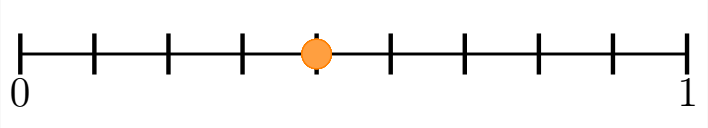
\includegraphics[width=180px]{../images/recta_num_frac4|9.png}   \hfill \fillin[\fbox{$\dfrac{ 4}{9 }$}][0in]
				\part 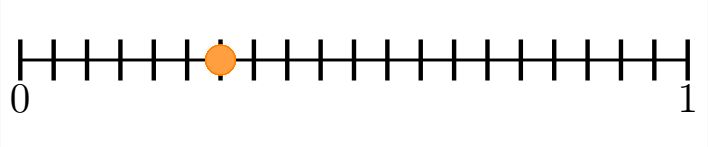
\includegraphics[width=180px]{../images/recta_num_frac6|20.png}  \hfill \fillin[\fbox{$\dfrac{ 6}{20}$}][0in]
				\part 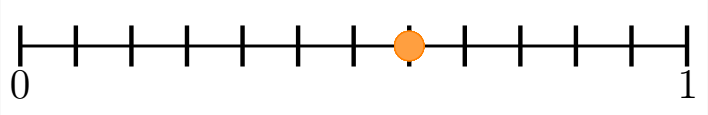
\includegraphics[width=180px]{../images/recta_num_frac7|12.png}  \hfill \fillin[\fbox{$\dfrac{ 7}{12}$}][0in]
				\part 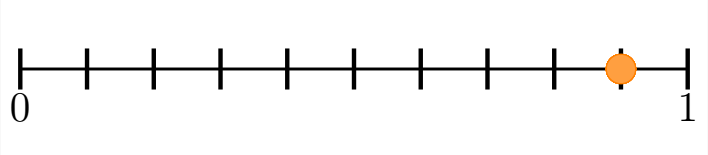
\includegraphics[width=180px]{../images/recta_num_frac9|10.png}  \hfill \fillin[\fbox{$\dfrac{ 9}{10}$}][0in]
				\part 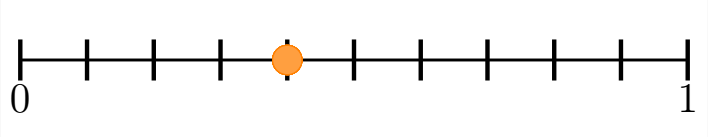
\includegraphics[width=180px]{../images/recta_num_frac4|10.png}  \hfill \fillin[\fbox{$\dfrac{ 4}{10}$}][0in]
				\part 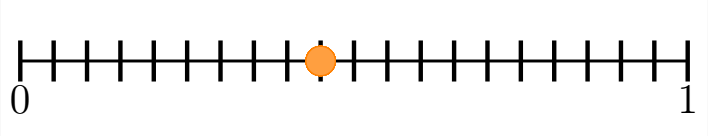
\includegraphics[width=180px]{../images/recta_num_frac9|20.png}  \hfill \fillin[\fbox{$\dfrac{ 9}{20}$}][0in]
				\part 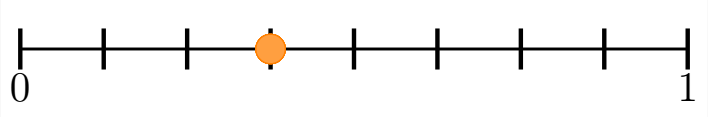
\includegraphics[width=180px]{../images/recta_num_frac3|8.png}   \hfill \fillin[\fbox{$\dfrac{ 3}{8 }$}][0in]
				\part 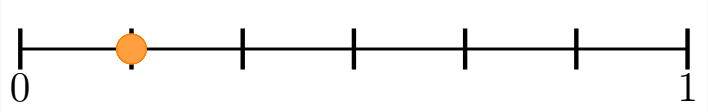
\includegraphics[width=180px]{../images/recta_num_frac1|6.png}   \hfill \fillin[\fbox{$\dfrac{ 1}{6 }$}][0in]
				\part 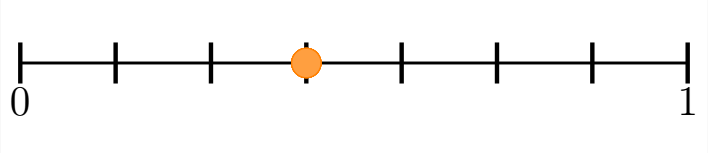
\includegraphics[width=180px]{../images/recta_num_frac3|7.png}   \hfill \fillin[\fbox{$\dfrac{ 3}{7 }$}][0in]
				\part 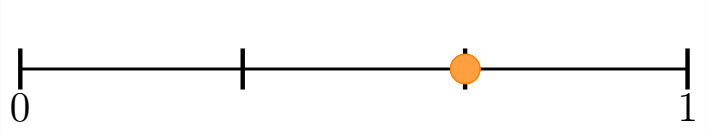
\includegraphics[width=180px]{../images/recta_num_frac2|3.png}   \hfill \fillin[\fbox{$\dfrac{ 2}{3 }$}][0in]
			\end{parts}
		\end{multicols}
	}

	\addcontentsline{toc}{subsubsection}{Conversión de fracciones}
	\subsubsection*{Conversión de fracciones}

	\questionboxed[2]{Convierte la siguientes fracciones mixtas a impropias y viseversa:

		\begin{multicols}{3}
			\begin{parts}
				\part $4\dfrac{2}{3}= $  \fillin[$\dfrac{14}{3}$][0in]\\
				\part $\dfrac{13}{3}= $  \fillin[$4\dfrac{1}{3}$][0in]\\
				\part $2\dfrac{3}{10}= $ \fillin[$\dfrac{23}{10}$][0in]\\
				\part $\dfrac{43}{10}= $ \fillin[$4\dfrac{3}{10}$][0in]\\
				\part $5\dfrac{1}{5}= $  \fillin[$\dfrac{26}{5}$][0in]\\
				\part $\dfrac{51}{5}= $  \fillin[$10\dfrac{1}{5}$][0in]\\
			\end{parts}
		\end{multicols}
	}

	\addcontentsline{toc}{subsection}{Simplificación de fracciones}
	\subsection*{Simplificación de fracciones}
	\addcontentsline{toc}{subsubsection}{Comparación de fracciones}
	\subsubsection*{Comparación de fracciones}

	\questionboxed[2]{Escribe sobre la línea el símbolo de mayor que ($>$), menor que ($<$), o igual ($=$) según corresponda.

		\begin{multicols}{5}
			\begin{parts}
				\part $\dfrac{2}{5}$ \fillin[$>$][0.5in] $\dfrac{1}{3}$\\[0.25em]
				\part $\dfrac{3}{4}$ \fillin[$<$][0.5in] $\dfrac{4}{5}$\\[0.25em]
				\part $\dfrac{2}{5}$ \fillin[$<$][0.5in] $\dfrac{2}{3}$\\[0.25em]
				\part $\dfrac{3}{2}$ \fillin[$=$][0.5in] $\dfrac{9}{6}$\\[0.25em]
				\part $\dfrac{5}{6}$ \fillin[$>$][0.5in] $\dfrac{4}{6}$\\[0.25em]
				\part $\dfrac{4}{3}$ \fillin[$>$][0.5in] $\dfrac{5}{4}$\\[0.25em]
				\part $\dfrac{1}{3}$ \fillin[$=$][0.5in] $\dfrac{9}{3}$\\[0.25em]
				\part $\dfrac{2}{3}$ \fillin[$<$][0.5in] $\dfrac{3}{2}$\\[0.25em]
				\part $\dfrac{3}{4}$ \fillin[$>$][0.5in] $\dfrac{2}{3}$\\[0.25em]
				\part $\dfrac{5}{6}$ \fillin[$>$][0.5in] $\dfrac{4}{5}$\\[0.25em]
			\end{parts}
		\end{multicols}
	}


	\addcontentsline{toc}{subsubsection}{Mínimo común múltiplo}
	\subsubsection*{Mínimo común múltiplo}
	\addcontentsline{toc}{subsubsection}{Máximo común divisor}
	\subsubsection*{Máximo común divisor}

	\questionboxed[2]{Calcula lo que se te pide en cada inciso:

		% \begin{multicols}{2}
		\begin{parts}
			% \part Encuentra el mínimo común múltiplo de 2 y 9.     	\hfill\fillin[El MCM de 2 y 9 es 18.][0in] \\
			% \part Encuentra el máximo común divisor de 5 y 15.     	\hfill\fillin[El MCD de 5 y 15 es 5.][0in] \\
			\part Encuentra el máximo común divisor de 24 y 56.   	\hfill\fillin[El MCD de 24 y 56 es 8.][0in] \\
			% \part Encuentra el máximo común divisor de 25 y 100.   	\hfill\fillin[El MCD de 25 y 100 es 25.][0in] \\
			\part Encuentra el máximo común divisor de 28 y 36.    	\hfill\fillin[El MCD de 28 y 36 es 4.][0in] \\
			\part Encuentra el mínimo común múltiplo de 4 y 10.     	\hfill\fillin[El MCM de 4 y 10 es 20.][0in] \\
			\part Encuentra el mínimo común múltiplo de 60 y 75.     	\hfill\fillin[El MCM de 60 y 75 es 300.][0in] \\
			% \part Encuentra el mínimo común múltiplo de 2, 6 y 4.  	\hfill\fillin[El MCM de 2, 6 y 4 es 12.][0in] \\
			\part Encuentra el máximo común divisor de 12 y 14.     	\hfill\fillin[El MCD de 12 y 14 es 2.][0in] \\
			\part Encuentra el mínimo común múltiplo de 12, 15 y 18.\hfill\fillin[El MCM de 12, 15 y 18 es 180.][0in] \\
		\end{parts}
		% \end{multicols}
	}

	\addcontentsline{toc}{subsubsection}{Simplificación de fracciones}
	\subsubsection*{Simplificación de fracciones}

	\questionboxed[2]{Simplifica a su mínima expresión las siguientes fracciones usando el máximo común divisor:

		\begin{multicols}{5}
			\begin{parts}
				\part $\dfrac{12}{48}= $  \fillin[$\dfrac{1}{4}$][0in]\\[0.5em]
				\part $\dfrac{6}{24}= $  \fillin[$\dfrac{1}{4}$][0in]\\[0.5em]
				\part $\dfrac{16}{36}= $  \fillin[$\dfrac{4}{9}$][0in]\\[0.5em]
				\part $\dfrac{4}{40}= $  \fillin[$\dfrac{1}{10}$][0in]\\[0.5em]
				\part $\dfrac{4}{20}= $  \fillin[$\dfrac{1}{5}$][0in]\\[0.5em]
				\part $\dfrac{2}{30}= $  \fillin[$\dfrac{1}{15}$][0in]\\[0.5em]
				\part $\dfrac{6}{36}= $  \fillin[$\dfrac{1}{6}$][0in]\\[0.5em]
				\part $\dfrac{5}{25}= $  \fillin[$\dfrac{1}{5}$][0in]\\[0.5em]
				\part $\dfrac{6}{30}= $  \fillin[$\dfrac{1}{5}$][0in]\\[0.5em]
				\part $\dfrac{2}{12}= $  \fillin[$\dfrac{1}{6}$][0in]\\[0.5em]
				\part $\dfrac{4}{16}= $  \fillin[$\dfrac{1}{4}$][0in]\\[0.5em]
				\part $\dfrac{15}{20}= $  \fillin[$\dfrac{3}{4}$][0in]\\[0.5em]
				\part $\dfrac{5}{50}= $  \fillin[$\dfrac{1}{10}$][0in]\\[0.5em]
				\part $\dfrac{6}{10}= $  \fillin[$\dfrac{3}{5}$][0in]\\[0.5em]
				\part $\dfrac{3}{18}= $  \fillin[$\dfrac{1}{6}$][0in]\\[0.5em]
			\end{parts}
		\end{multicols}
	}

	
	\addcontentsline{toc}{subsubsection}{Fracciones equivalentes}
	\subsubsection*{Fracciones equivalentes}

	\questionboxed[2]{Indica si las siguientes fracciones son equivalentes o no:

		\begin{multicols}{2}
			\begin{parts}

				\part $\dfrac{1}{2}=\dfrac{4}{6}$\qquad
				\begin{oneparcheckboxes}
					\choice Sí
					\CorrectChoice No
				\end{oneparcheckboxes}

				\part $\dfrac{4}{5}=\dfrac{8}{10}$\qquad
				\begin{oneparcheckboxes}
					\CorrectChoice Sí
					\choice No
				\end{oneparcheckboxes}

				\part $\dfrac{1}{8}=\dfrac{4}{16}$\qquad
				\begin{oneparcheckboxes}
					\choice Sí
					\CorrectChoice No
				\end{oneparcheckboxes}

				\part $\dfrac{1}{5}=\dfrac{5}{10}$\qquad
				\begin{oneparcheckboxes}
					\choice Sí
					\CorrectChoice No
				\end{oneparcheckboxes}

				% \part $\dfrac{1}{10}=\dfrac{3}{30}$\qquad
				% \begin{oneparcheckboxes}
				% 	\CorrectChoice Sí
				% 	\choice No
				% \end{oneparcheckboxes}

				% \part $\dfrac{1}{4}=\dfrac{2}{4}$\qquad
				% \begin{oneparcheckboxes}
				% 	\choice Sí
				% 	\CorrectChoice No
				% \end{oneparcheckboxes}

				% \part $\dfrac{1}{5}=\dfrac{10}{25}$\qquad
				% \begin{oneparcheckboxes}
				% 	\choice Sí
				% 	\CorrectChoice No
				% \end{oneparcheckboxes}

				% \part $\dfrac{3}{2}=\dfrac{12}{8}$\qquad
				% \begin{oneparcheckboxes}
				% 	\CorrectChoice Sí
				% 	\choice No
				% \end{oneparcheckboxes}

				% \part $\dfrac{3}{6}=\dfrac{1}{3}$\qquad
				% \begin{oneparcheckboxes}
				% 	\choice Sí
				% 	\CorrectChoice No
				% \end{oneparcheckboxes}

				% \part $\dfrac{18}{12}=\dfrac{9}{4}$\qquad
				% \begin{oneparcheckboxes}
				% 	\choice Sí
				% 	\CorrectChoice No
				% \end{oneparcheckboxes}
			\end{parts}
		\end{multicols}
	}


	

	\addcontentsline{toc}{subsection}{Suma y resta de fracciones}
	\subsection*{Suma y resta de fracciones}
	\addcontentsline{toc}{subsubsection}{Simplificación de fracciones}
	\subsubsection*{Simplificación de fracciones}
	\addcontentsline{toc}{subsubsection}{Suma y resta con denominadores iguales}
	\subsubsection*{Suma y resta con denominadores iguales}
	\addcontentsline{toc}{subsubsection}{Suma y resta denominadores diferentes 1}
	\subsubsection*{Suma y resta denominadores diferentes 1}
	\addcontentsline{toc}{subsubsection}{Suma y resta denominadores diferentes 2}
	\subsubsection*{Suma y resta denominadores diferentes 2}

	\questionboxed[2]{Realiza las siguientes operaciones de suma y resta de fracciones:

		\begin{multicols}{3}
			\begin{parts}
				\part $\dfrac{3}{5}+\dfrac{4}{5}=$ \fillin[$\dfrac{7}{5} = 1\dfrac{2}{5}$][0in] \\[1em]
				\part $\dfrac{3}{10}+\dfrac{4}{5}=$ \fillin[$\dfrac{11}{10} = 1\dfrac{1}{10}$][0in] \\[1em]
				\part $\dfrac{9}{10}+\dfrac{2}{3}=$ \fillin[$1\dfrac{17}{30}$][0in] \\[1em]
				\part $\dfrac{13}{6}-\dfrac{5}{6}=$ \fillin[$\dfrac{8}{6}=\dfrac{4}{3}$][0in] \\[1em]
				\part $1\dfrac{1}{2}+1\dfrac{2}{3}=$ \fillin[$3\dfrac{1}{6}$][0in] \\[1em]
				\part $\dfrac{3}{4}-\dfrac{2}{5}=$ \fillin[$\dfrac{7}{20}$][0in] \\[1em]
				\part $\dfrac{5}{6}+\dfrac{1}{12}=$ \fillin[$\dfrac{11}{12}$][0in] \\[1em]
				\part $\dfrac{12}{7}-\dfrac{5}{7}=$ \fillin[$\dfrac{7}{7}=1$][0in] \\[1em]
				\part $\dfrac{2}{3}-\dfrac{2}{5}=$ \fillin[$\dfrac{4}{15}$][0in] \\[1em]
				\part $2\dfrac{1}{2}-1\dfrac{1}{3}=$ \fillin[$1\dfrac{1}{6}$][0in] \\[1em]
				\part $\dfrac{1}{3}-\dfrac{1}{4}=$ \fillin[$\dfrac{1}{12}$][0in] \\[1em]
				\part $1\dfrac{1}{8}+1\dfrac{7}{8}=$ \fillin[$2\dfrac{8}{8} = 3$][0in] \\[1em]
				\part $\dfrac{3}{8}+\dfrac{7}{10}=$ \fillin[$\dfrac{43}{40} = 1\dfrac{3}{40}$][0in] \\[1em]
				\part $\dfrac{3}{4}-\dfrac{1}{8}=$ \fillin[$\dfrac{5}{8}$][0in] \\[1em]
				\part $3\dfrac{3}{4}-2\dfrac{2}{3}=$ \fillin[$1\dfrac{1}{12}$][0in] \\[1em]
			\end{parts}
		\end{multicols}
	}

	%% \addcontentsline{toc}{subsubsection}{Resolución de problemas}
	%% \subsubsection*{Resolución de problemas}

	\addcontentsline{toc}{subsection}{Multiplicación y división de fracciones}
	\subsection*{Multiplicación y división de fracciones}
	\addcontentsline{toc}{subsubsection}{Multiplicación de fracciones}
	\subsubsection*{Multiplicación de fracciones}
	\addcontentsline{toc}{subsubsection}{División de fracciones}
	\subsubsection*{División de fracciones}
	\addcontentsline{toc}{subsubsection}{Multiplicación y división 1}
	\subsubsection*{Multiplicación y división 1}
	\addcontentsline{toc}{subsubsection}{Multiplicación y división 2}
	\subsubsection*{Multiplicación y división 2}


	\questionboxed[2]{Realiza las siguientes operaciones de multiplicación y división de fracciones (Expresa tu resultadocomo una \textbf{fracción simplificada}):

		\begin{multicols}{4}
			\begin{parts}
				\part $\dfrac{7}{9}\times\dfrac{12}{17}=$ \fillin[$\dfrac{28}{51}$][0in]   \\[1em]
				\part $\dfrac{2}{7}\divisionsymbol\dfrac{2}{5}=$ \fillin[$\dfrac{5}{7}$][0in]   \\[1em]
				\part $3\times\dfrac{5}{4}=$ \fillin[$\dfrac{15}{4}$][0in]   \\[1em]
				\part $1\dfrac{1}{4}\times 4\dfrac{5}{8}=$ \fillin[$\dfrac{185}{32}$][0in]   \\[1em]
				\part $\dfrac{5}{6}\times\dfrac{4}{5}=$ \fillin[$\dfrac{2}{3}$][0in]   \\[1em]
				\part $\dfrac{4}{7}\divisionsymbol\dfrac{5}{6}=$ \fillin[$\dfrac{24}{35}$][0in]   \\[1em]
				\part $\dfrac{7}{6}\times 6=$ \fillin[$\dfrac{21}{2}$][0in]   \\[1em]
				\part $3\dfrac{1}{3}\times 2\dfrac{2}{5}=$ \fillin[$8$][0in]   \\[1em]
				\part $\dfrac{3}{7}\times\dfrac{5}{6}=$ \fillin[$\dfrac{5}{14}$][0in]   \\[1em]
				\part $\dfrac{7}{8}\divisionsymbol\dfrac{5}{4}=$ \fillin[$\dfrac{7}{10}$][0in]   \\[1em]
				\part $\dfrac{2}{5}\divisionsymbol 5=$ \fillin[$\dfrac{2}{25}$][0in]   \\[1em]
				\part $6\dfrac{1}{2}\divisionsymbol 1\dfrac{5}{7}=$ \fillin[$\dfrac{91}{24}$][0in]   \\[1em]
				\part $\dfrac{5}{8}\times\dfrac{4}{5}=$ \fillin[$\dfrac{1}{2}$][0in]   \\[1em]
				\part $\dfrac{6}{7}\divisionsymbol\dfrac{1}{3}=$ \fillin[$\dfrac{18}{7}$][0in]   \\[1em]
				\part $4\divisionsymbol\dfrac{3}{5}=$ \fillin[$\dfrac{20}{3}$][0in]   \\[1em]
				\part $2\dfrac{2}{3}\divisionsymbol 1\dfrac{3}{4}=$ \fillin[$\dfrac{32}{21}$][0in]   \\[1em]
			\end{parts}
		\end{multicols}
	}

	%% \addcontentsline{toc}{subsubsection}{Resolución de problemas}
	%% \subsubsection*{Resolución de problemas}

	\addcontentsline{toc}{subsection}{Porcentajes}
	\subsection*{Porcentajes}
	\addcontentsline{toc}{subsubsection}{Porcentajes a decimales}
	\subsubsection*{Porcentajes a decimales}

	\questionboxed[2]{Escribe los siguientes porcentajes como números decimales:

		\begin{multicols}{4}
			\begin{parts}
				\part $14\%=$ \fillin[\fbox{0.14}][0cm] 
				\part $73\%=$ \fillin[\fbox{0.73}][0cm] 
				\part $15\%=$ \fillin[\fbox{0.15}][0cm] 
				\part $85\%=$ \fillin[\fbox{0.85}][0cm] 
				\part $91\%=$ \fillin[\fbox{0.91}][0cm] 
				\part $19\%=$ \fillin[\fbox{0.19}][0cm] 
				\part $ 9\%=$ \fillin[\fbox{0.09}][0cm] 
				\part $42\%=$ \fillin[\fbox{0.42}][0cm] 
				\part $25\%=$ \fillin[\fbox{0.25}][0cm] 
				\part $ 3\%=$ \fillin[\fbox{0.03}][0cm] 
				\part $ 8\%=$ \fillin[\fbox{0.08}][0cm] 
				\part $ 2\%=$ \fillin[\fbox{0.02}][0cm] 
			\end{parts}
		\end{multicols}
	}

	\addcontentsline{toc}{subsubsection}{Decimales a porcentajes}
	\subsubsection*{Decimales a porcentajes}

	\questionboxed[2]{Escribe el porcentaje que representa cada número decimal:

		\begin{multicols}{3}
			\begin{parts}
				\part $0.44=$ \fillin[$44\%$][0in]
				\part $0.092=$ \fillin[$9.2\%$][0in]
				\part $0.05=$ \fillin[$5\%$][0in]
				\part $0.25=$ \fillin[$25\%$][0in]
				\part $0.33=$ \fillin[$33\%$][0in]
				\part $0.209=$ \fillin[$20.9\%$][0in]
			\end{parts}
		\end{multicols}
	}

	%% \addcontentsline{toc}{subsubsection}{50\%, 25\%, 10\% y 1\%}
	%% \subsubsection*{50\%, 25\%, 10\% y 1\%}


	\addcontentsline{toc}{subsubsection}{Porcentajes de cantidades}
	\subsubsection*{Porcentajes de cantidades}

	\questionboxed[2]{Calcula los porentajes de los siguientes números:

		\begin{multicols}{2}
			\begin{parts}
				\part ¿Cuál es el 80\% de 660?   \hfill \fillin[\fbox{528}][0cm]
				\part ¿Cuál es el 20\% de 50?    \hfill \fillin[\fbox{10}][0cm]
				\part ¿Cuál es el 50\% de 862?   \hfill \fillin[\fbox{431}][0cm]
				\part ¿Cuál es el 30\% de 300?   \hfill \fillin[\fbox{90}][0cm]
				\part ¿Cuál es el 20\% de 415?   \hfill \fillin[\fbox{83}][0cm]
				\part ¿Cuál es el 12\% de 338?   \hfill \fillin[\fbox{40.56}][0cm]
				\part ¿Cuál es el 15\% de 711?   \hfill \fillin[\fbox{106.65}][0cm]
				\part ¿Cuál es el 80\% de 1260?  \hfill \fillin[\fbox{1008}][0cm]
			\end{parts}
		\end{multicols}
	}

	\addcontentsline{toc}{subsubsection}{Resolución de problemas}
	\subsubsection*{Resolución de problemas}

	\questionboxed[2]{Resuelve los siguientes problemas:

	\begin{multicols}{2}
		\begin{parts}
			\part El costo de una camisa es de \$800 pesos, si se les hace un descuento del 20\%, ¿cuánto pagaré en total por la camisa?

			\begin{solutionbox}{1.8cm}
				\[\$800\times 20\%=\$160\]
				\[\$800-\$160=\$640\]
			\end{solutionbox}

			\part El 24\% de los habitantes de un pueblo tienen menos de 30 años. ¿Cuántos habitantes tiene el pueblo si hay 120 jóvenes menores de 30 años?

			\begin{solutionbox}{1.8cm}
				\[\dfrac{120\times 100\%}{24\%}=500\]
			\end{solutionbox}
		\end{parts}
	\end{multicols}
	}
\end{questions}
\end{document}